\documentclass[]{article}

\usepackage{geometry}
\usepackage{subcaption}
\usepackage{graphicx}
\usepackage{minted}
\usepackage{hyperref}
\usepackage{lipsum}
\usepackage{wrapfig}
\usepackage{mathtools}
\usepackage{braket}

\geometry{a4paper}
\hypersetup{
colorlinks
}

%opening
\title{Sperimentando con diverse \\decomposizioni di una formula logica}
\author{Davide Camino}

\begin{document}

\maketitle

\begin{abstract}
	In questi esperimenti trasformiamo una formula logica prima in un circuito digitale, poi in un problema di ottimizzazione infine tentiamo di trovare una soluzione al problema di ottimizzazione con vari metodi. Lo scopo degli esperimenti è valutare se diverse traduzioni in circuito digitale (usando set di porte logiche diverse) o diverse traduzioni in problemi di ottimizzazione (usando diverse forme energetiche a parita di gate) impattano la qualità delle soluzioni del problema di ottimizzazione.
	
	Nella Sezione~\ref{sec:setup} vengono presentati la configurazione sperimentale, la formula logica di partenza, i diversi circuiti logici e le funzioni di energia adottate. La Sezione~\ref{sec:results} riporta i risultati ottenuti e un breve commento. Infine, la Sezione~\ref{sec:limits} discute i limiti dello studio e propone alcuni spunti per sviluppi futuri.
\end{abstract}

\section{Configurazione sperimentale}\label{sec:setup}
\subsection{Formula logica}
\begin{wrapfigure}{r}{.5\linewidth}
	\centering
	\vspace{-.5cm}
	\begin{minipage}{.8\linewidth}
		\begin{minted}[]{verilog}
module sat (
input  wire A,
input  wire B,
input  wire C,
output wire Y
);

	assign Y = C & ~(A | B);

endmodule
		\end{minted}
	\end{minipage}
	
\end{wrapfigure}
La formula logica di partenza è:
\begin{equation}
	Y = C \land \neg(A \lor B).
\end{equation}
La formula è volutamente semplice, così da consentire di individuare facilmente un assegnamento che la soddisfi. È stata inoltre scelta in modo che tale assegnamento sia unico. Di conseguenza, una volta tradotta la formula in un problema di ottimizzazione, lo spazio delle soluzioni presenta un unico minimo globale.

La formula è stata codificata direttamente in Verilog per mantenere un controllo puntuale sui bit utilizzati e consentirne la trasformazione in diversi circuiti logici mediante \emph{Yosys}. Il listato a destra mostra una possibile codifica della formula in Verilog.
\subsection{Circuiti digitali}
La compilazione del programma Verilog in un circuito digitale è stata effettuata con Yosys\footnote{\url{https://yosyshq.net/yosys/}}. Yosys è un software di sintesi hardware articolato e ricco di funzionalità, che esegue diverse fasi di compilazione e semplificazione del circuito. Le opzioni di compilazione possono essere specificate in un file di configurazione, solitamente denominato \texttt{synth.ys}.

Per realizzare gli esperimenti sono stati utilizzati due componenti del processo di compilazione di Yosys:
\begin{itemize}
	\item ABC\footnote{\url{https://github.com/berkeley-abc/abc}}: un insieme di strumenti per l'ottimizzazione logica a grana fine e il mapping su LUT. In questi esperimenti ABC viene utilizzato per stabilire quali porte siano ammesse nel circuito digitale finale. Ad esempio, aggiungendo al file \texttt{synth.ys} il comando \texttt{abc -g AND,XOR}, le sole porte logiche che possono comparire nel circuito finale sono \texttt{AND}, \texttt{XOR} e \texttt{NOT} (quest'ultima è sempre inclusa);
	\item Techmap: una fase di mapping tecnologico che sostituisce le celle del progetto con implementazioni specificate in un file sorgente Verilog. In questo caso Techmap viene utilizzato per definire porte logiche personalizzate, come la porta \texttt{TOFFOLI}. Dopo l'esecuzione di ABC, viene definita una corrispondenza per convertire le porte generate nelle porte desiderate.
\end{itemize}

Sono stati esaminati tre circuiti con diverse combinazioni di porte logiche, mostrati nella Figura~\ref{fig:circs}.

\begin{figure}
	\centering
	\begin{minipage}{0.48\textwidth}
		\vspace{-5cm}
		\begin{subfigure}{\textwidth}
			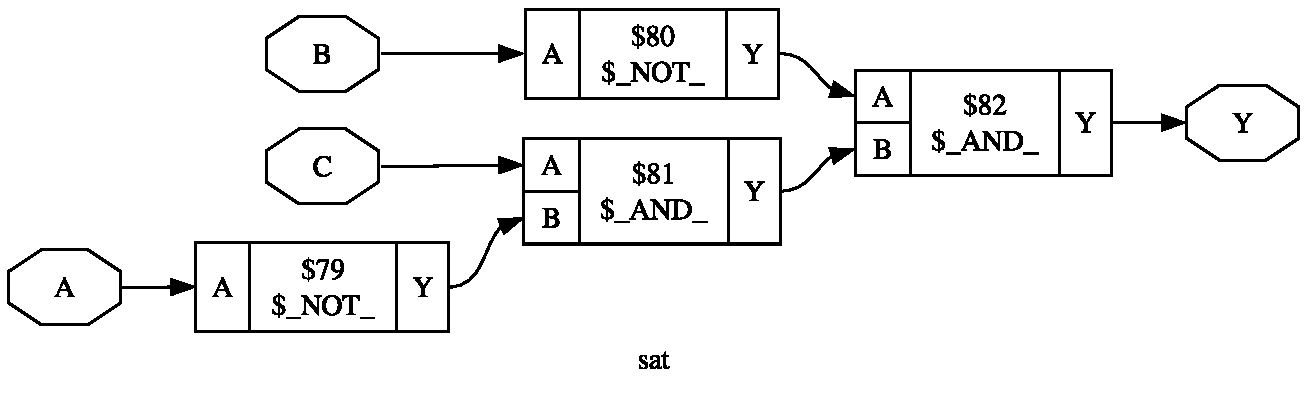
\includegraphics[width=\textwidth]{Pictures/not_and}
			\caption{Sole porte \texttt{NOT} e \texttt{AND}}
			\label{fig:circ_and}
		\end{subfigure}
		\begin{subfigure}{\textwidth}
			\vspace{.5cm}
			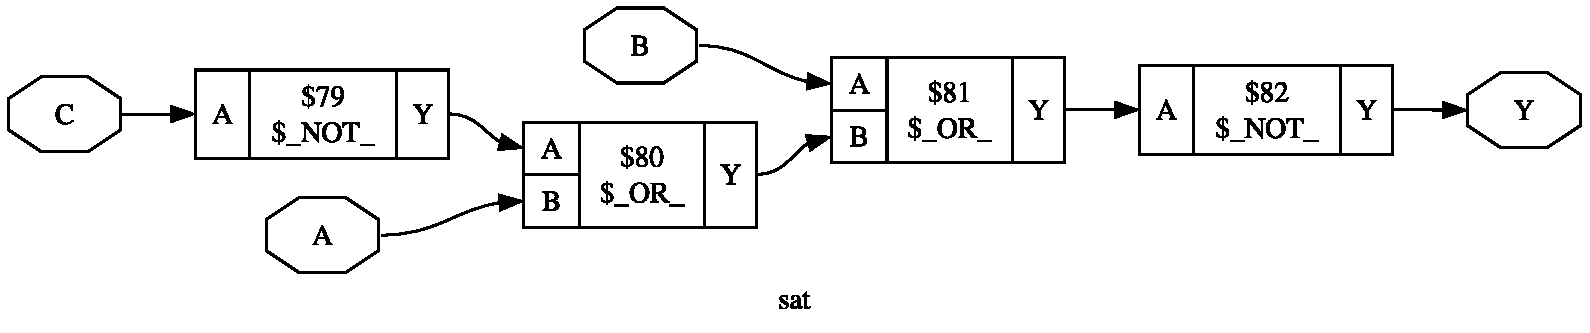
\includegraphics[width=\textwidth]{Pictures/not_or}
			\caption{Sole porte \texttt{NOT} e \texttt{OR}}
			\label{fig:circ_or}
		\end{subfigure}
	\end{minipage}
	\hfill
	\begin{subfigure}{0.48\textwidth}
		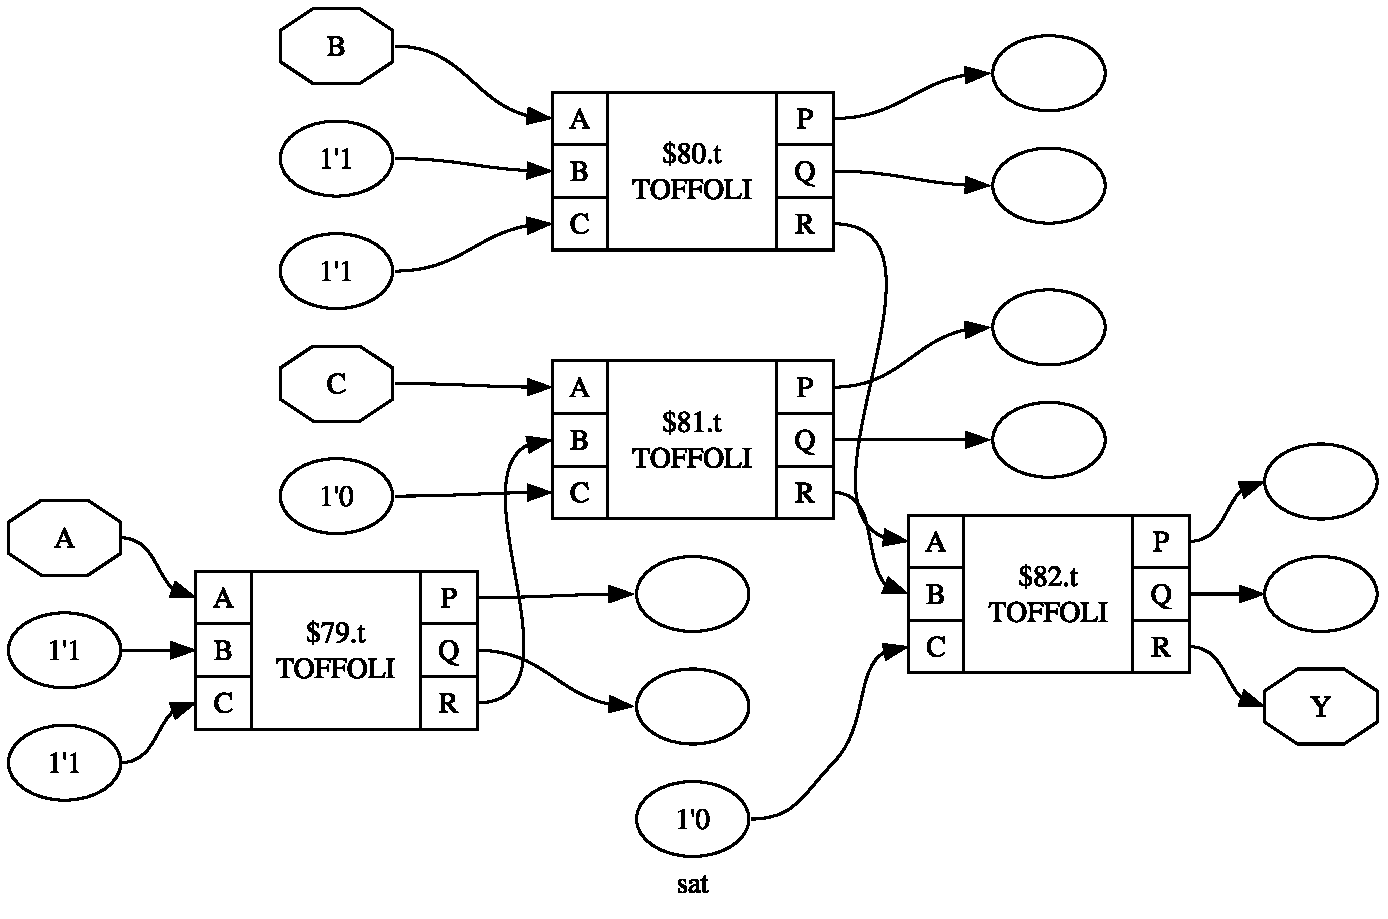
\includegraphics[width=\textwidth]{Pictures/toffoli}
		\caption{Sole porte \texttt{TOFFOLI}}
		\label{fig:circ_tof}
	\end{subfigure}
	\caption{Circuiti esaminati}
	\label{fig:circs}
\end{figure}
\subsection{Funzioni di energia}
A ogni porta logica è associata una funzione pseudobooleana che assegna un'energia a ciascuna configurazione dei bit in ingresso e in uscita. Tutte le configurazioni compatibili con la tavola di verità della porta corrispondono a minimi globali dell'energia. Questo consente di tradurre il vincolo imposto dalla porta logica in un problema di minimizzazione. La funzione di energia è espressa come un polinomio; la funzione pseudobooleana che rappresenta l'intero circuito si ottiene sommando i polinomi associati alle singole porte.

Di seguito sono riportati i polinomi associati a ciascuna porta. Poiché il problema è formulato in forma Ising, ogni variabile soddisfa $var \in \set{+1, -1}$; per convenzione, $+1$ rappresenta il valore di verità \texttt{True} e $-1$ il valore \texttt{False}. Le lettere maiuscole indicano i valori dei bit in ingresso ($A$, $B$, $C$) e in uscita ($Y$) dalle porte, mentre le lettere minuscole indicano variabili ancillari. I polinomi~\ref{eqn:and} e ~\ref{eqn:and_anc} definiscono due versioni della porta \texttt{AND}, rispettivamente senza e con variabili ancillari. Nei risultati vengono quindi presentate e discusse due formulazioni dello stesso circuito digitale, ottenute utilizzando le due versioni della porta.

L'introduzione di una variabile ancillare nella formulazione della porta \texttt{AND} mira ad aumentare la separazione tra il minimo globale della funzione pseudobooleana e il livello energetico immediatamente superiore. Nel problema QUBO o Ising, ciò corrisponde ad ampliare il divario energetico tra lo stato ground e il primo stato eccitato. 

La motivazione teorica di questa scelta risiede nel teorema adiabatico, che impone vincoli sul tempo di annealing legati al divario energetico tra lo stato ground e il primo stato eccitato: al diminuire di tale divario, aumentano i tempi richiesti per mantenere l'evoluzione adiabatica.

{
	\footnotesize
	\begin{align}
		\texttt{NOT}:&3 AY\\
		\texttt{OR}:&+A +B -2 Y +AB -2 AY -2 BY\\
		\texttt{AND}:&-A -B +2 Y +AB -2 AY -2 BY\label{eqn:and} \\
		\texttt{AND}\textnormal{-ancillary}:&-A -B + Y + x + AB- AY- Ax -BY-Bx -Yx\label{eqn:and_anc}\\
		\texttt{TOFFOLI:}& -A-B-C-Y+3 x + 2 y+AB-2Ax-2Bx+CY-Cx-2Cy-Yx-2Yy+2xy
	\end{align}
}

\subsection{Esecuzione degli esperimenti}
Per eseguire gli esperimenti sono stati sviluppati la libreria Python \emph{OpenQUOPS}\footnote{\url{https://github.com/DavideCamino/OpenQUOPS}}; alcune utility\footnote{\url{https://github.com/DavideCamino/Reports/tree/main/Gates_to_Ising/code/utility}} estrarre dai file generati da Yosys una lista di gates, e per trasformare questa lista di porte logiche prima in un polinomio e successivamente in un problema in forma Ising; infine uno script\footnote{\url{https://github.com/DavideCamino/Reports/tree/main/Gates_to_Ising/code}} per automatizzare l'esecuzione delle prove. Gli esperimenti sono stati eseguiti su Fedarchs\footnote{FEDARCHS cluster running on OpenStack available to $\alpha$ group \& friends.}. 

OpenQUOPS (Open Quadratic Unconstrained Optimization Problem Solver) consente di definire e manipolare problemi di ottimizzazione in forma QUBO o Ising. La libreria si interfaccia con la libreria Python \emph{qubovert}\footnote{\url{https://qubovert.readthedocs.io/en/latest/index.html}}, permettendo di importare problemi definiti in qubovert e di esportare quelli definiti in OpenQUOPS. OpenQUOPS integra inoltre diversi solver per problemi QUBO o Ising. Al momento sono disponibili la ricerca bruteforce, il simulated annealing, il simulated quantum annealing e il QAOA simulato.

I test hanno riguardato tutti i metodi probabilistici disponibili in OpenQUOPS. Per ciascun metodo e ciascun circuito sono state eseguite 30 prove indipendenti, calcolando poi la media e la deviazione standard dei risultati raccolti. Ogni prova prevedeva $2^{16}$ samples. Per QAOA è stato costruito un circuito a 2 livelli ed è stata adottata una policy di restarting dell'ottimizzazione dei parametri: ogni run prevede $20$ ottimizzazioni indipendenti, tra le quali viene selezionata quella che consente di ottenere l'energia più bassa.

\section{Risultati}\label{sec:results}
I risultati sono riportati nella Figura~\ref{fig:results}, organizzata come una tabella: le colonne corrispondono ai metodi di risoluzione e le righe ai diversi circuiti. In ciascun grafico della Figura~\ref{fig:results}, il secondo punto rappresenta il numero di osservazioni dell'assegnamento corretto ed è evidenziato in grassetto rispetto agli altri.
La disponibilità di numerose porte logiche rende pressoché illimitate le combinazioni con cui decomporre una formula. Tuttavia, già le quattro decomposizioni considerate consentono di formulare alcune osservazioni:
\begin{itemize}
	\item I risultati ottenuti con QAOA seguono un andamento simile a quelli del simulated quantum annealing, ma presentano un rumore molto maggiore;
	\item In assenza di variabili ancillari, e quindi a parità di numero di variabili utilizzate, la combinazione \texttt{AND-NOT} sembra fornire risultati migliori della combinazione \texttt{OR-NOT};
	\item A parità di porte logiche, l'impiego di polinomi senza variabili ancillari consente di ottenere risultati di qualità superiore. In questo caso, l'aumento del numero di variabili sembra introdurre più rumore di quanto se ne riesca a ridurre aumentando la separazione energetica tra lo stato ground e il primo stato eccitato;
	\item Probabilmente per ragioni analoghe, il caso caratterizzato dal maggior rumore è quello del circuito composto da sole porte \texttt{TOFFOLI}, che presenta anche il maggior numero di variabili.
\end{itemize}

\section{Limitazioni}\label{sec:limits}
Lo studio presenta le seguenti limitazioni, che suggeriscono possibili direzioni di approfondimento:
\begin{itemize}
	\item Le combinazioni di porte logiche esaminate sono molto poche;
	\item Manca una definizione della porta \texttt{AND} con due variabili ancillari;
	\item Anche la porta \texttt{OR} può essere formulata mediante un polinomio con una o due variabili ancillari, ma queste formulazioni non sono state considerate;
	\item Non è stata condotta un'analisi sistematica di tutte le porte per individuare e selezionare quelle che forniscono i risultati migliori;
	\item Quando l'insieme delle porte è generato da Yosys utilizzando solo ABC, il circuito è ottimizzato per usare meno porte possibili. Quando invece si ricorre a Techmap, la conversione in porte \texttt{TOFFOLI} avviene mediante una sostituzione uno a uno, senza considerare possibili raggruppamenti. Ad esempio, una porta \texttt{AND} seguita da una porta \texttt{XOR} potrebbe essere sostituita da un'unica porta \texttt{TOFFOLI} che ne realizzi la funzione complessiva; Techmap genera invece due porte, ciascuna delle quali implementa una singola porta del circuito originale.
\end{itemize}

\newgeometry{left=1cm, right=1cm, bottom=2cm}

\begin{figure}
	\centering
	\begin{subfigure}{0.375\textwidth}
		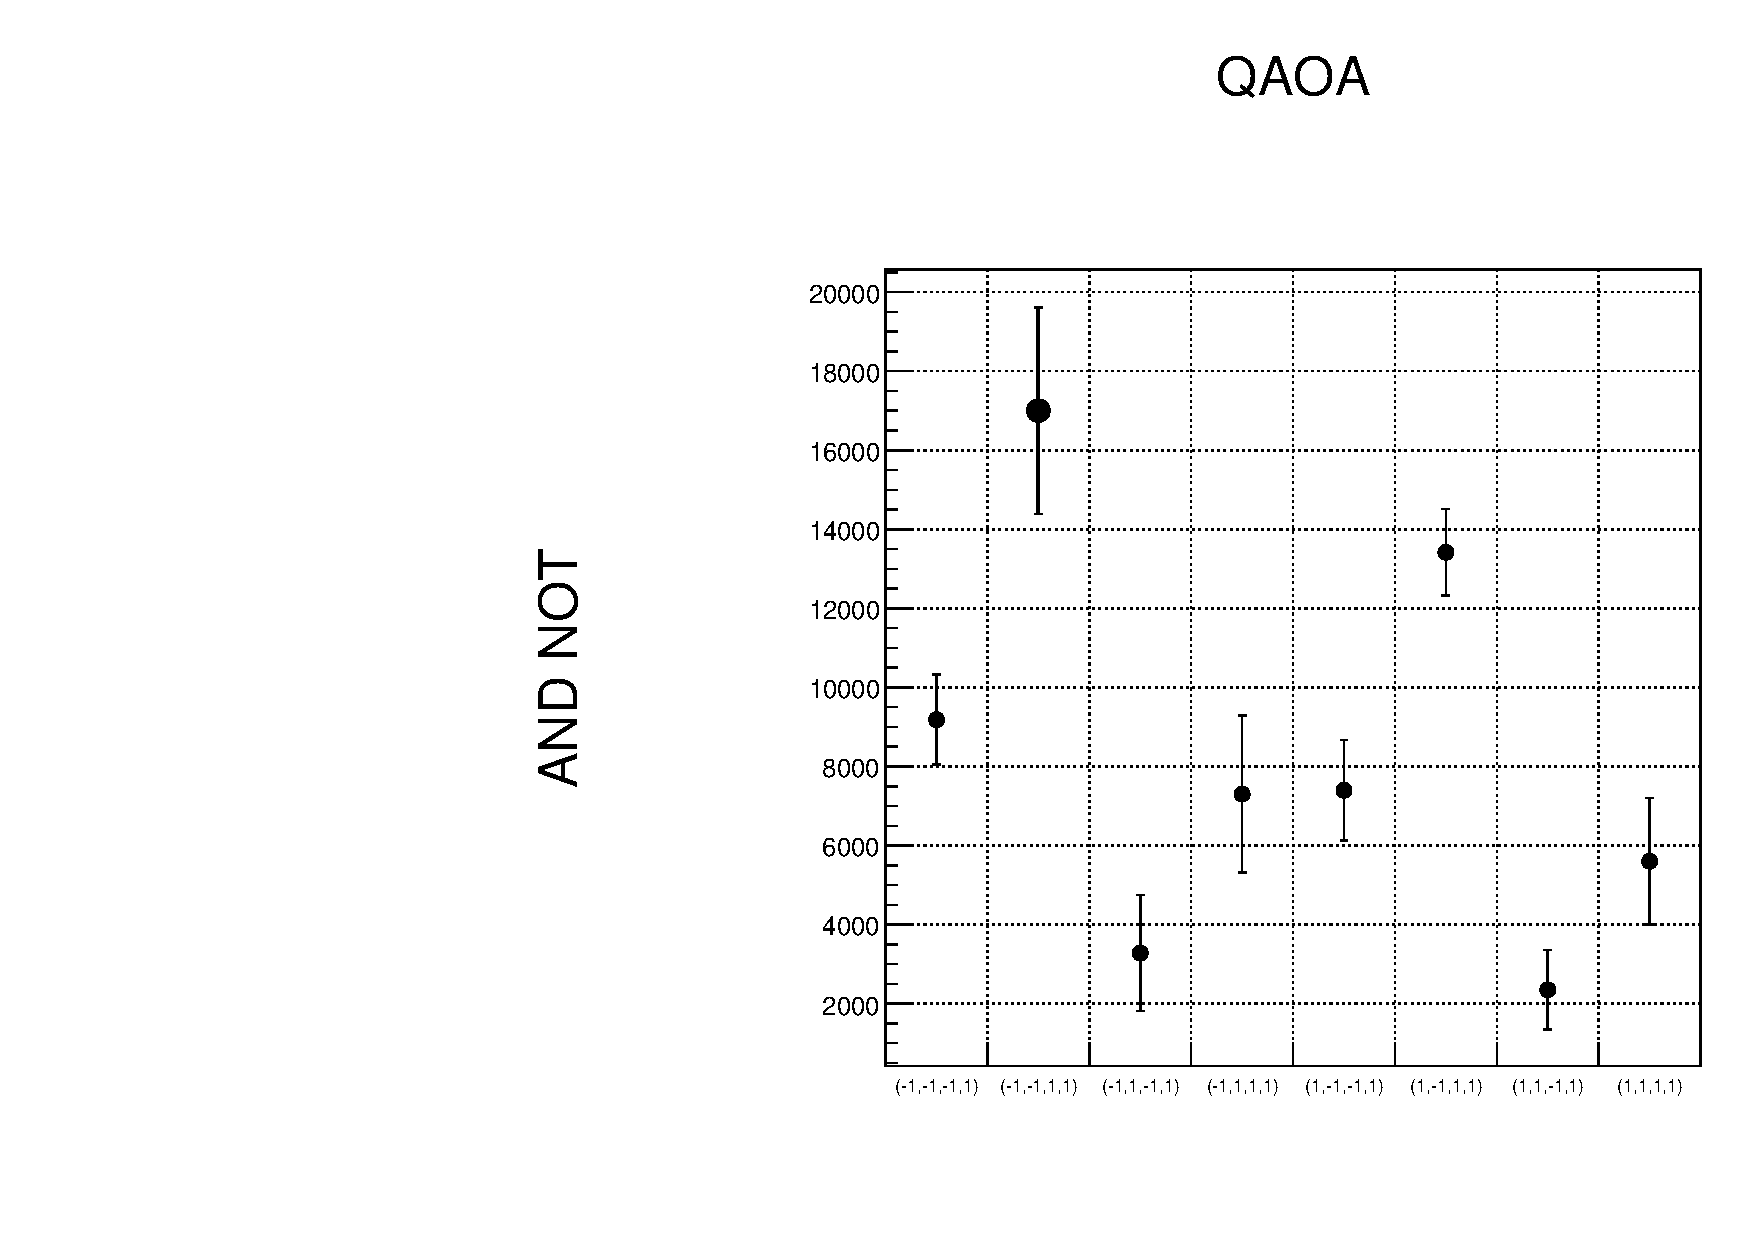
\includegraphics[width=\textwidth]{Pictures/0}
	\end{subfigure}
	\hspace{-1.5cm}
	\begin{subfigure}{0.375\textwidth}
		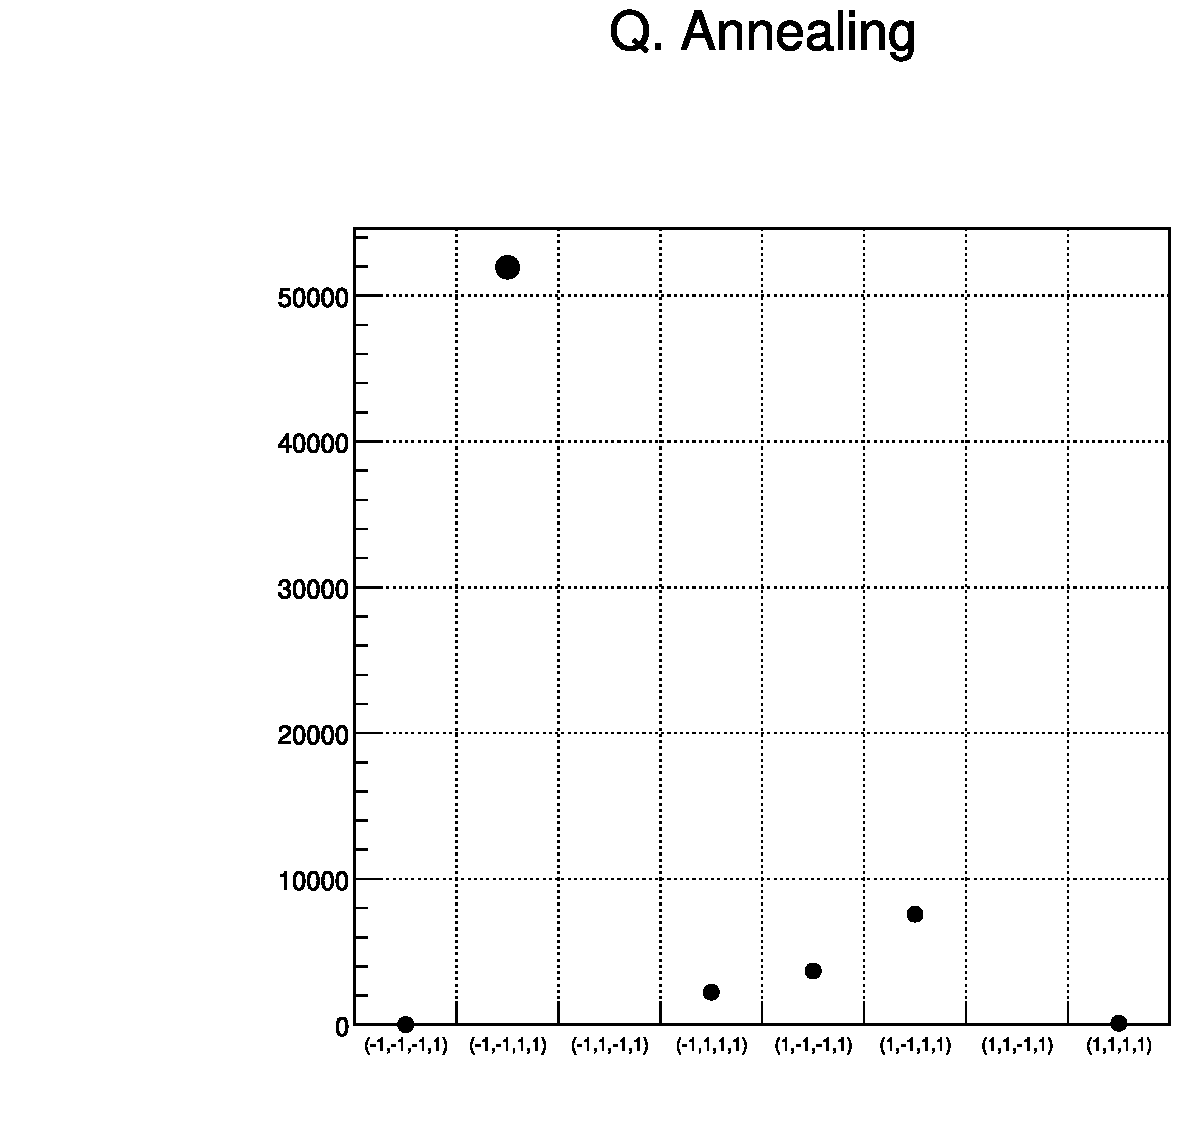
\includegraphics[width=\textwidth]{Pictures/1}
	\end{subfigure}
	\hspace{-1.5cm}
	\begin{subfigure}{0.375\textwidth}
		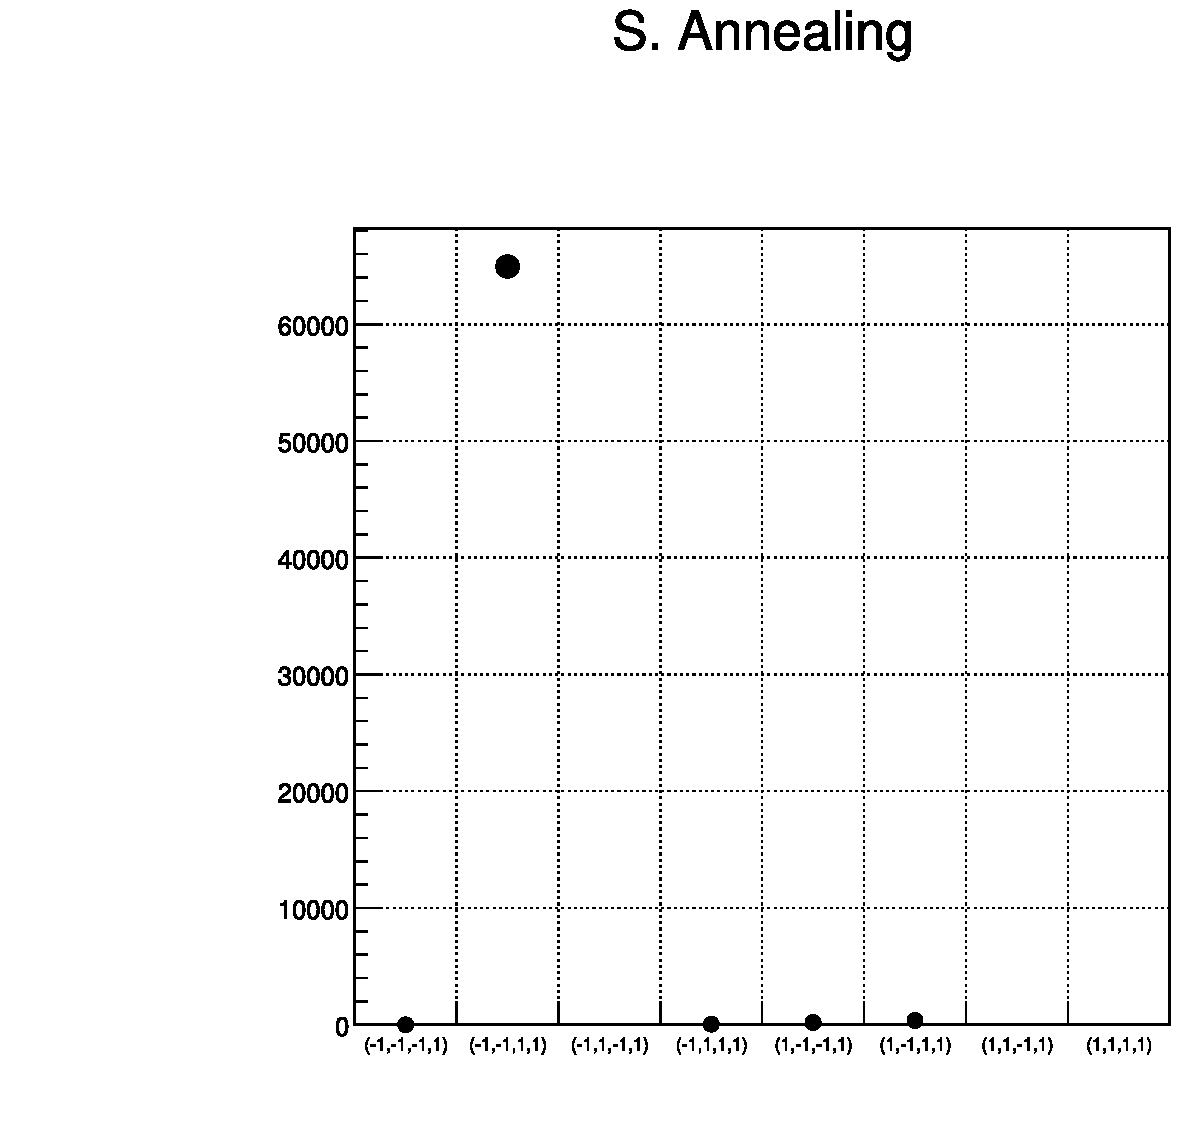
\includegraphics[width=\textwidth]{Pictures/2}
	\end{subfigure}
	
	\vspace{-1.5cm}
	
	\begin{subfigure}{0.375\textwidth}
		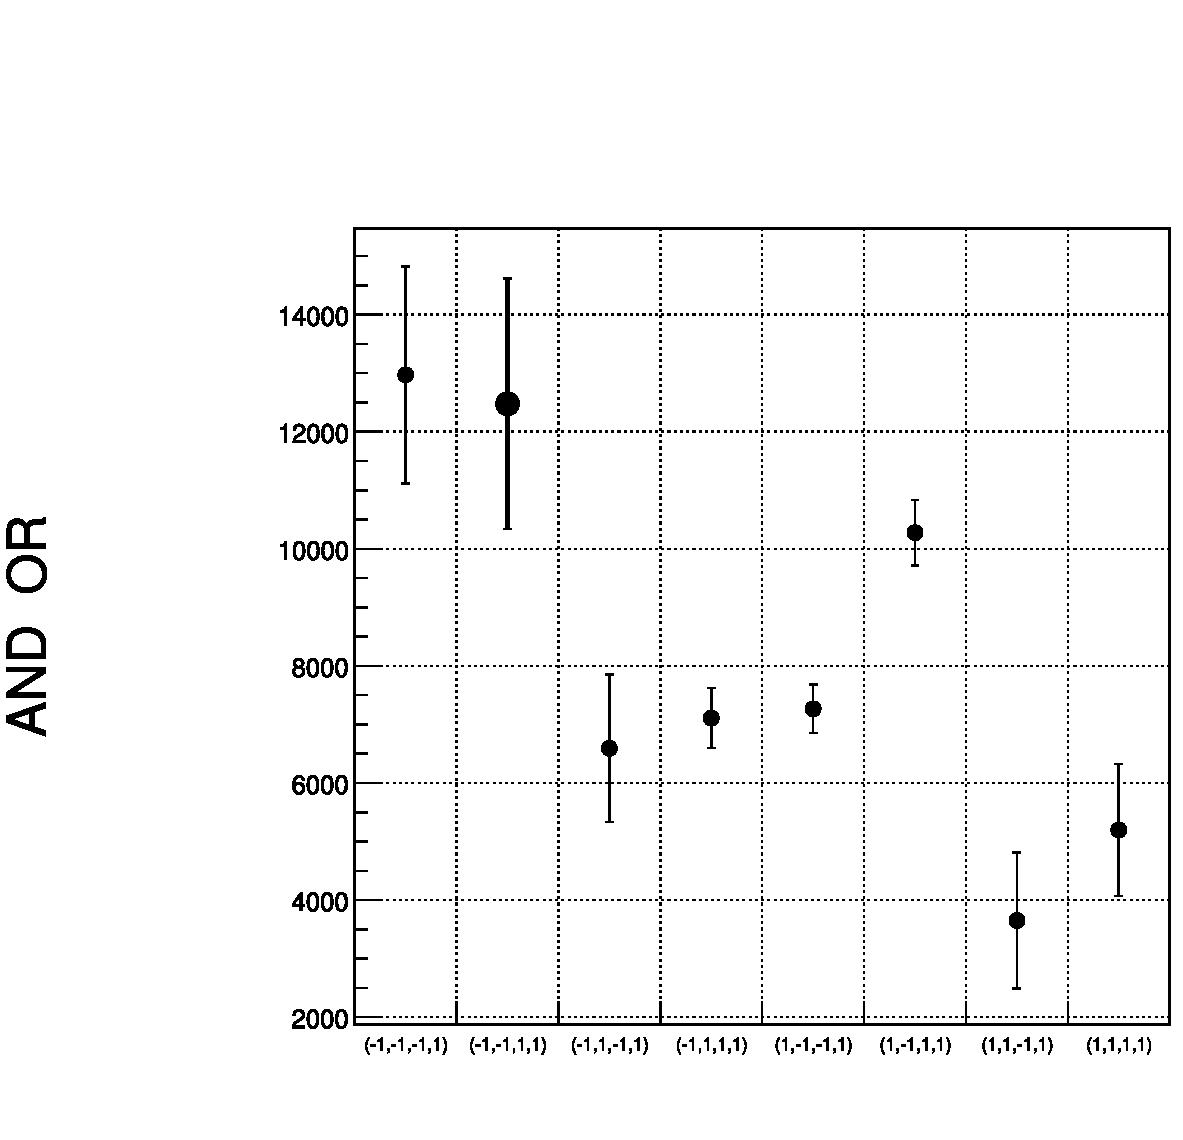
\includegraphics[width=\textwidth]{Pictures/3}
	\end{subfigure}
	\hspace{-1.5cm}
	\begin{subfigure}{0.375\textwidth}
		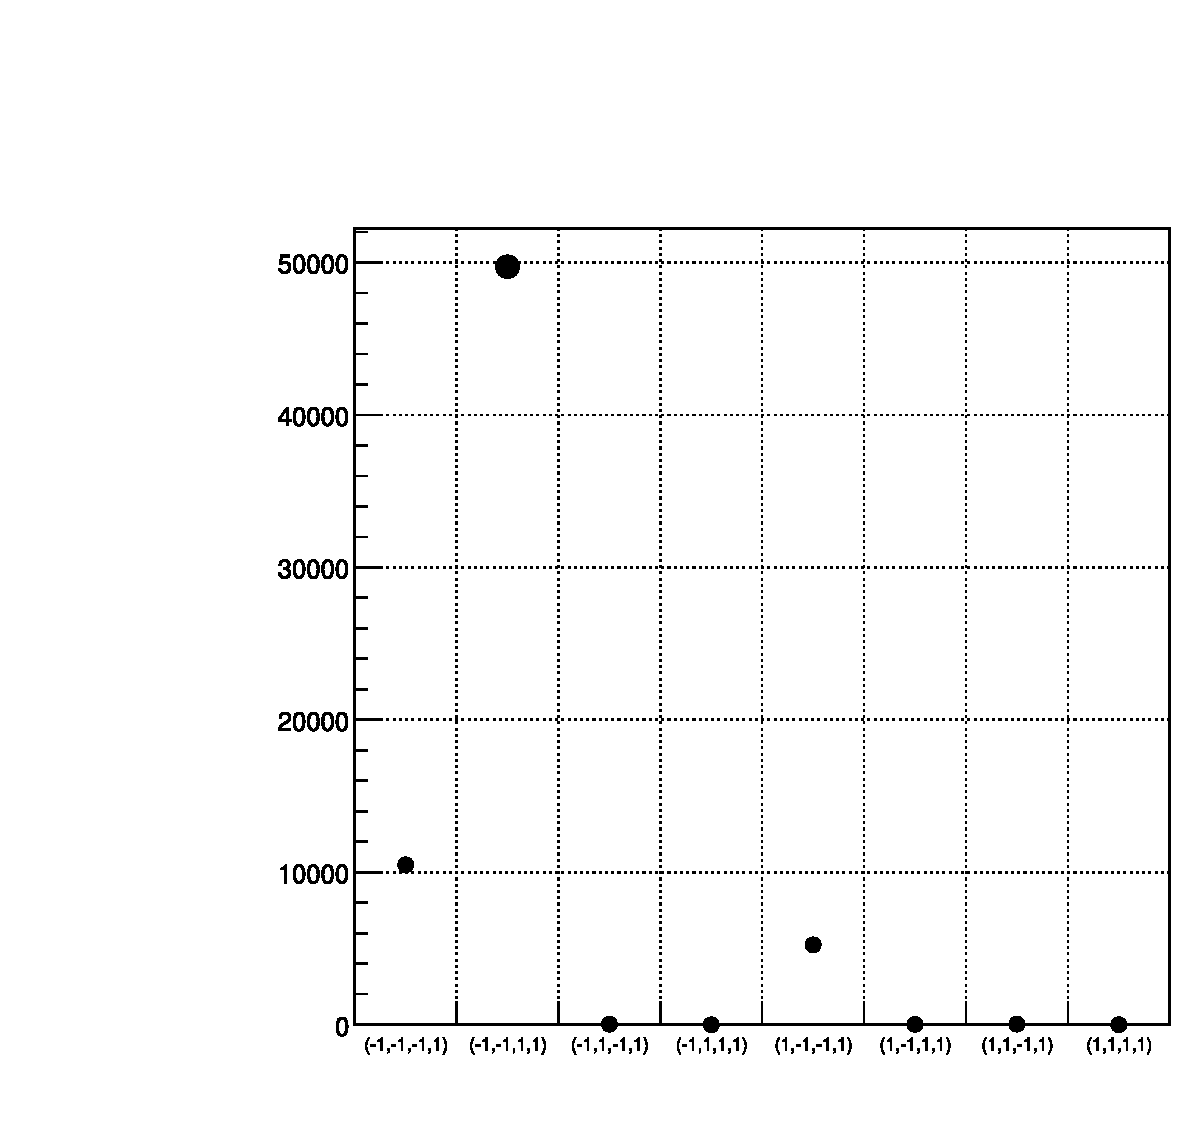
\includegraphics[width=\textwidth]{Pictures/4}
	\end{subfigure}
	\hspace{-1.5cm}
	\begin{subfigure}{0.375\textwidth}
		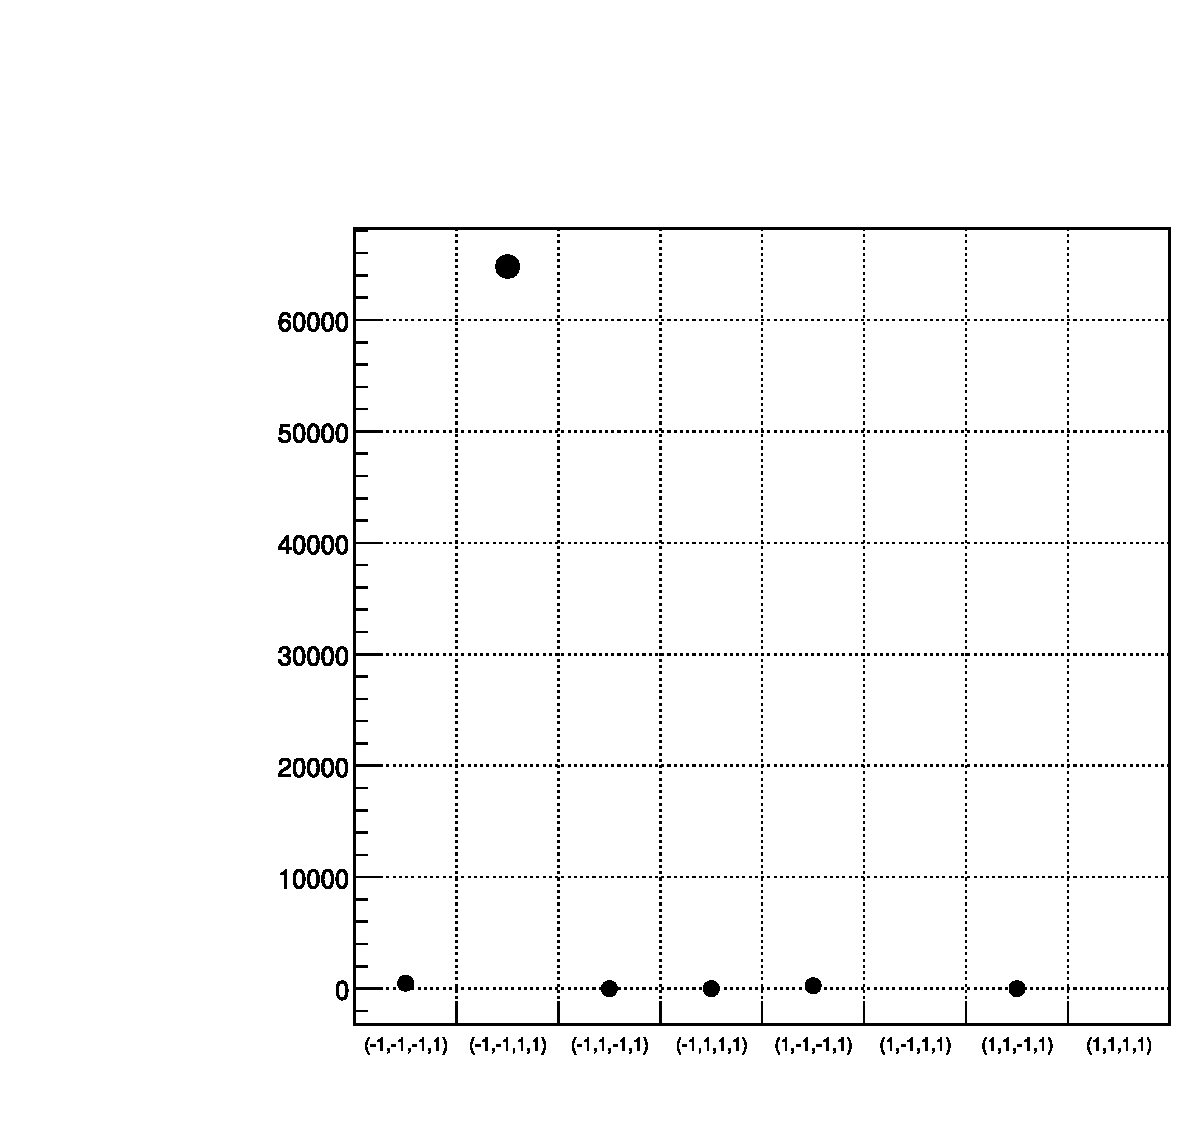
\includegraphics[width=\textwidth]{Pictures/5}
	\end{subfigure}
	
	\vspace{-1.5cm}
	
	\begin{subfigure}{0.375\textwidth}
		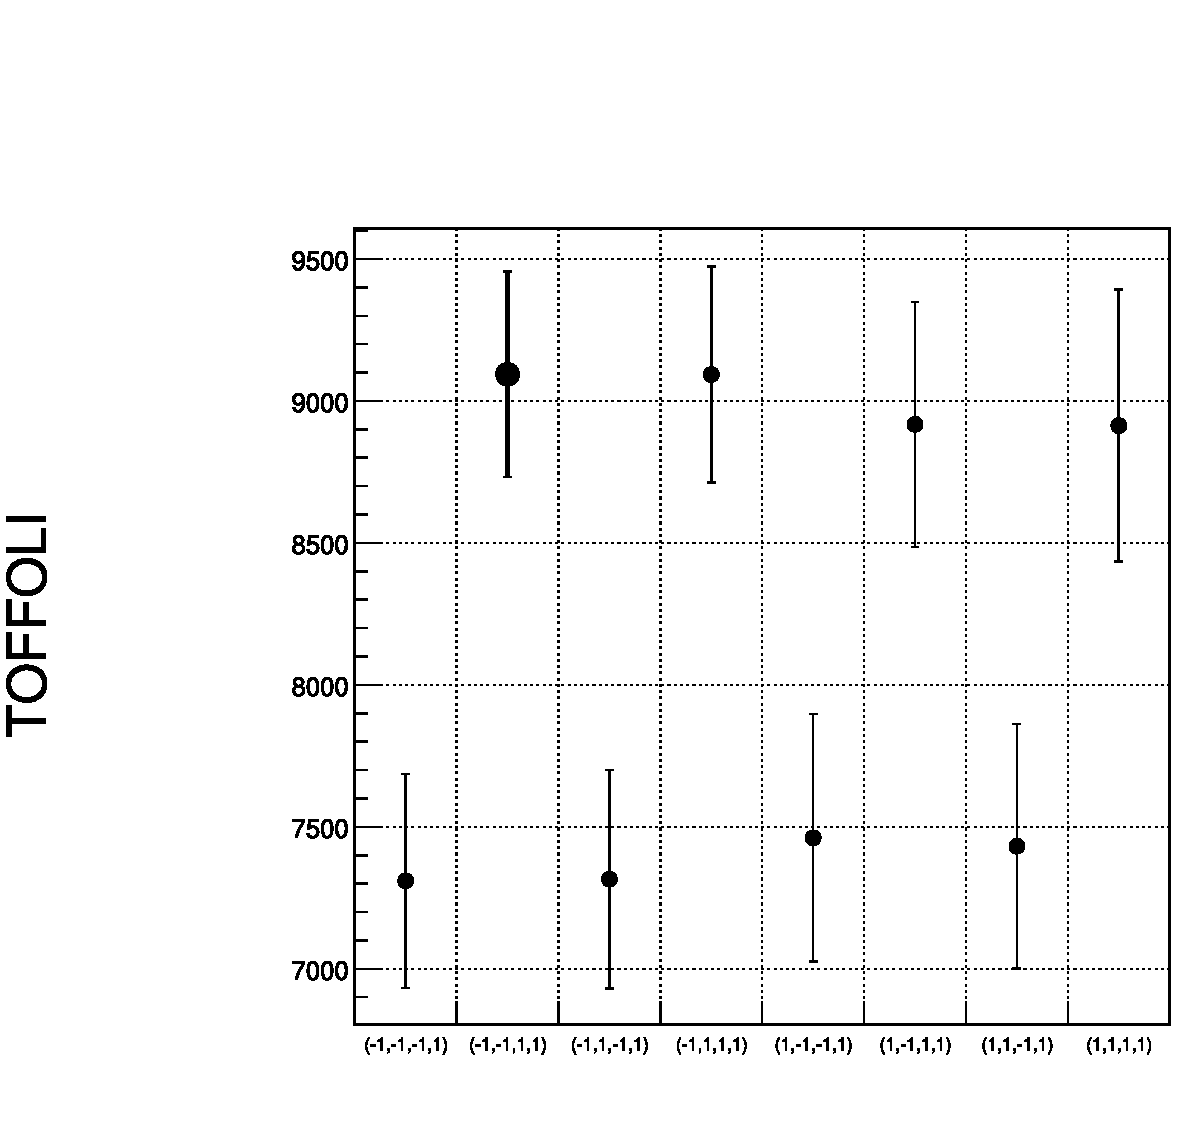
\includegraphics[width=\textwidth]{Pictures/6}
	\end{subfigure}
	\hspace{-1.5cm}
	\begin{subfigure}{0.375\textwidth}
		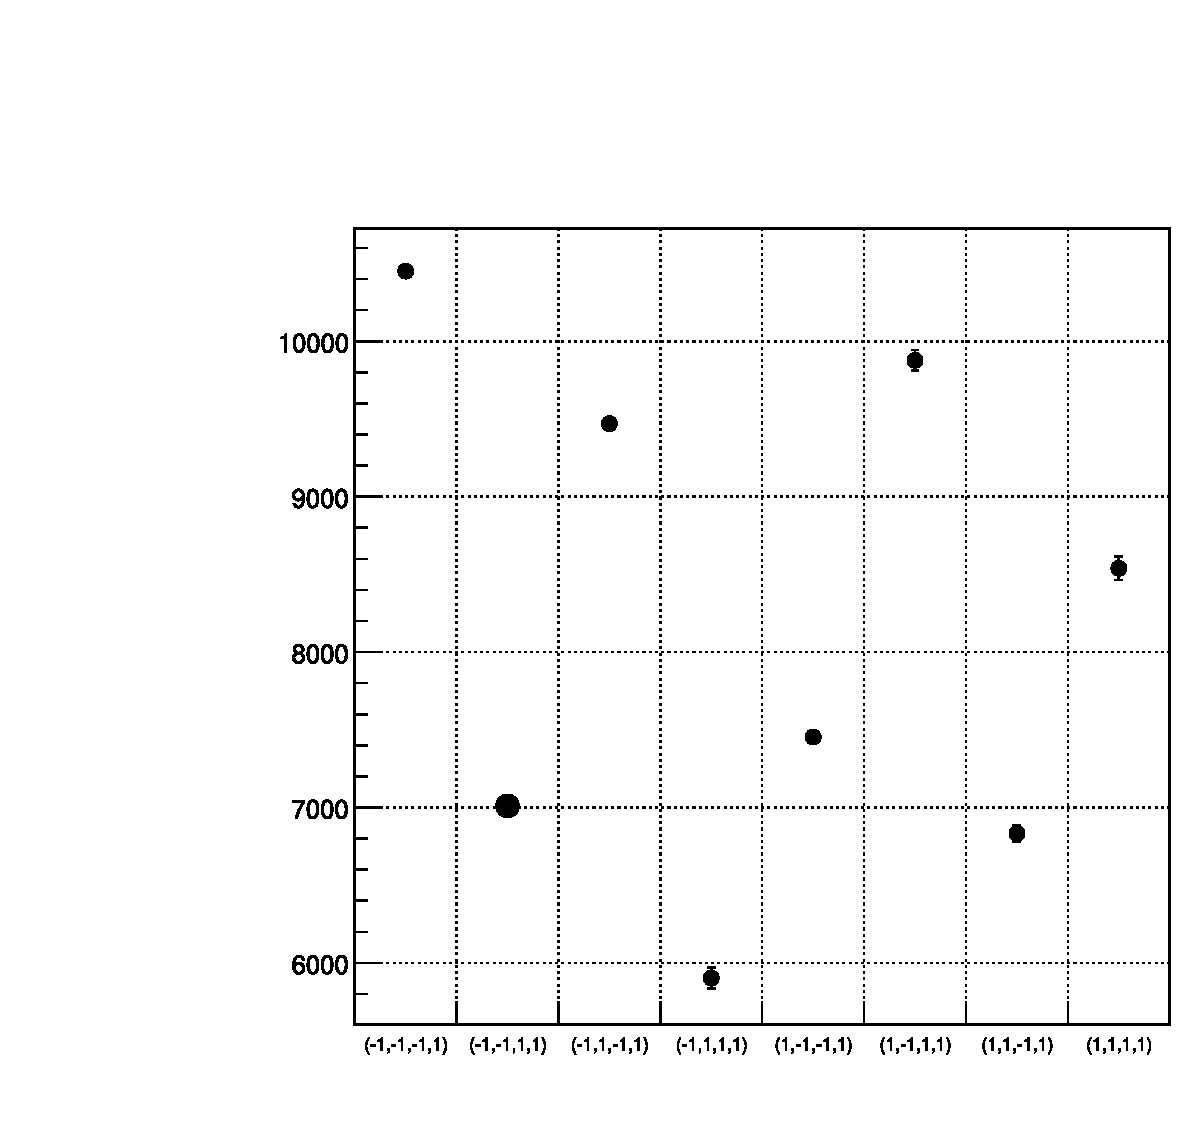
\includegraphics[width=\textwidth]{Pictures/7}
	\end{subfigure}
	\hspace{-1.5cm}
	\begin{subfigure}{0.375\textwidth}
		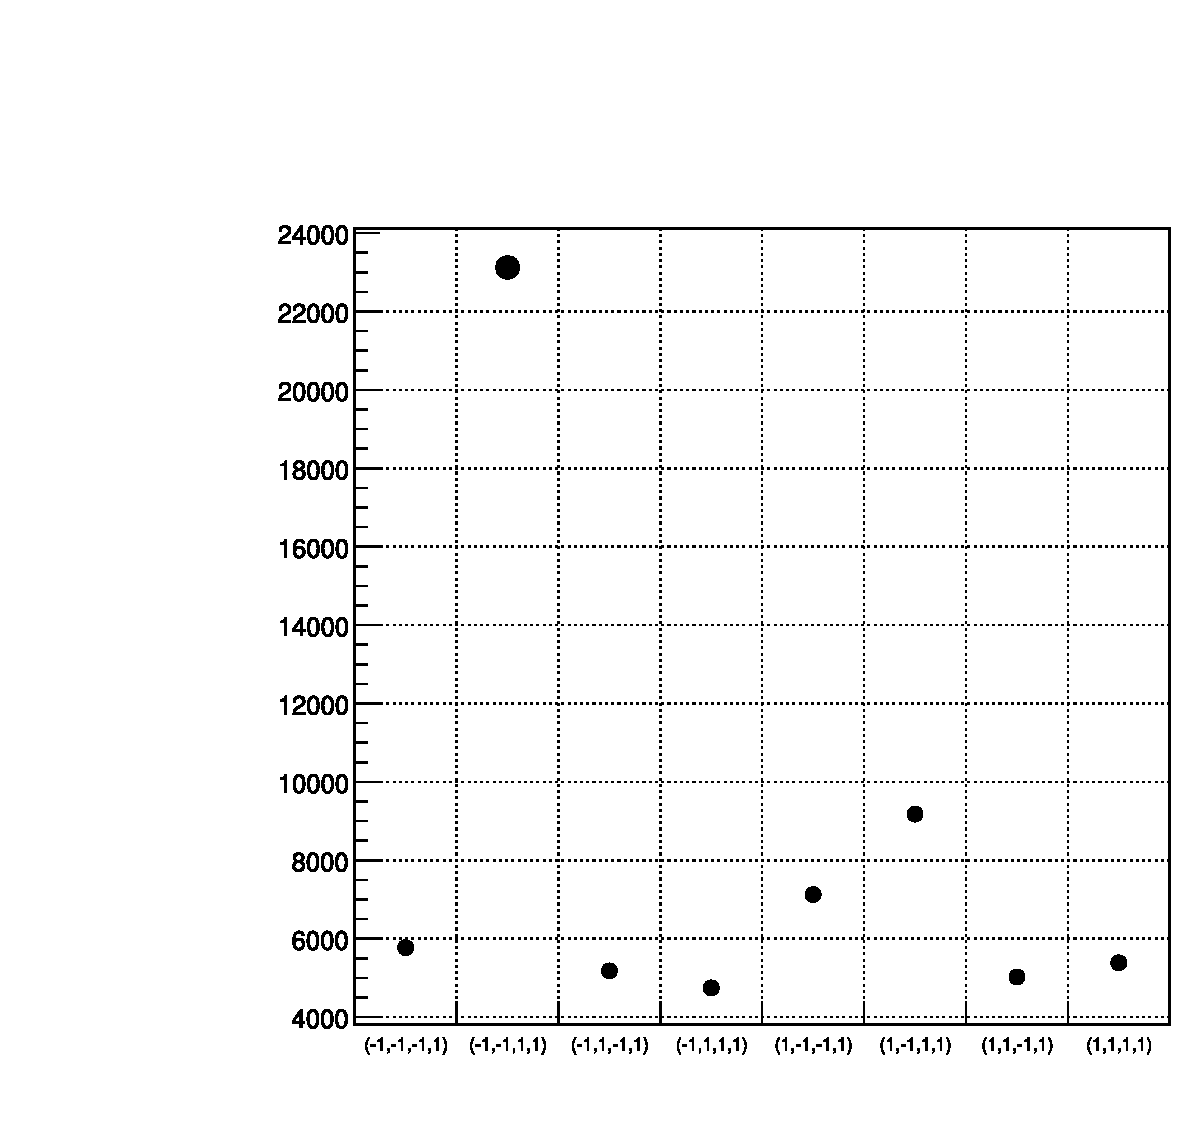
\includegraphics[width=\textwidth]{Pictures/8}
	\end{subfigure}
	
	\vspace{-1.5cm}
	
	\begin{subfigure}{0.375\textwidth}
		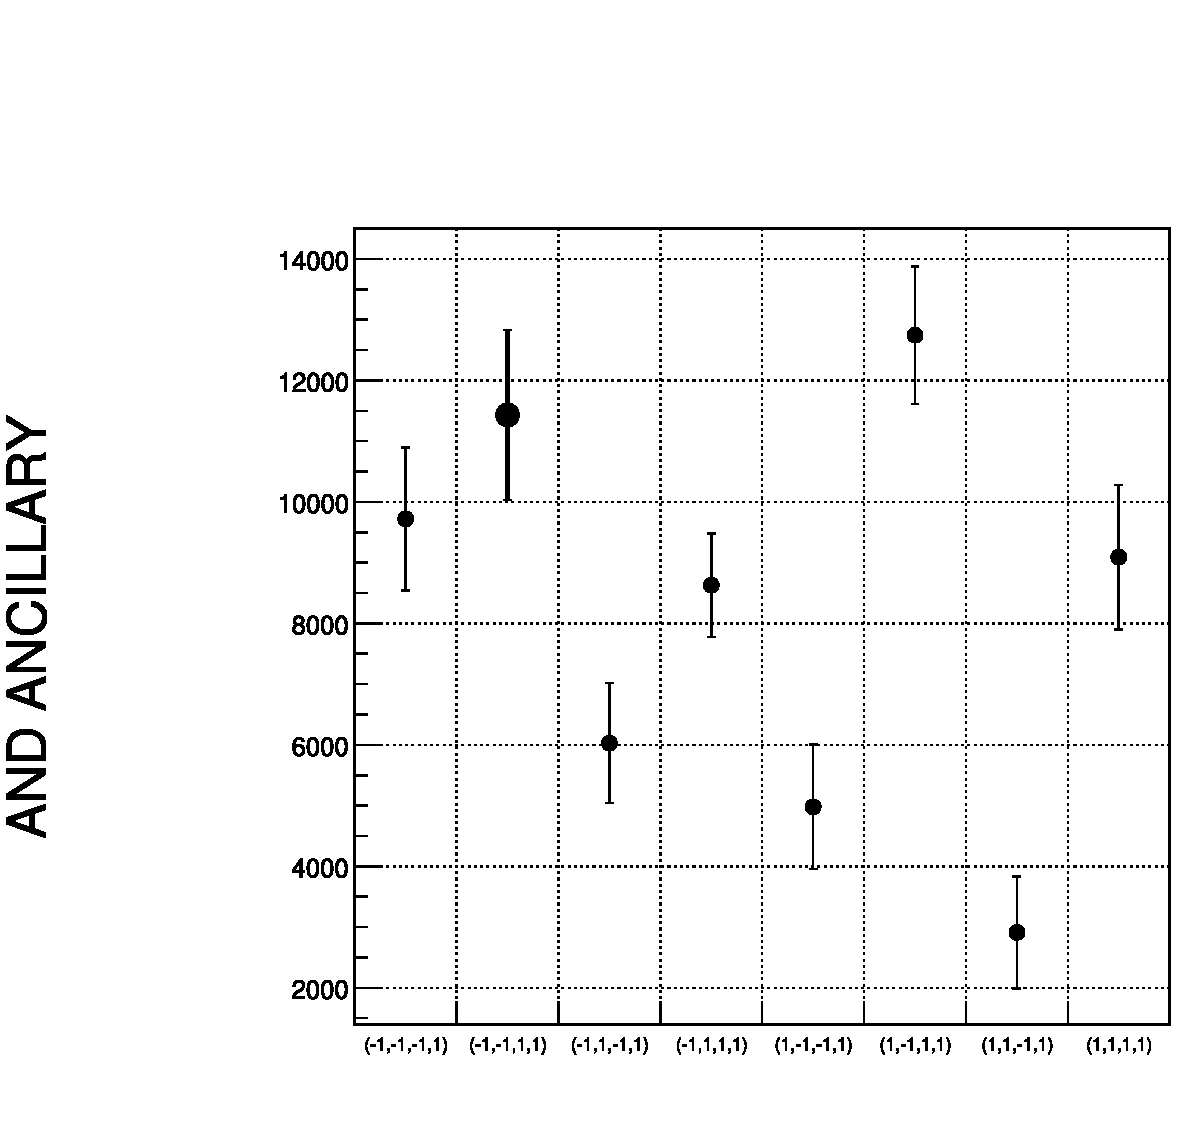
\includegraphics[width=\textwidth]{Pictures/9}
	\end{subfigure}
	\hspace{-1.5cm}
	\begin{subfigure}{0.375\textwidth}
		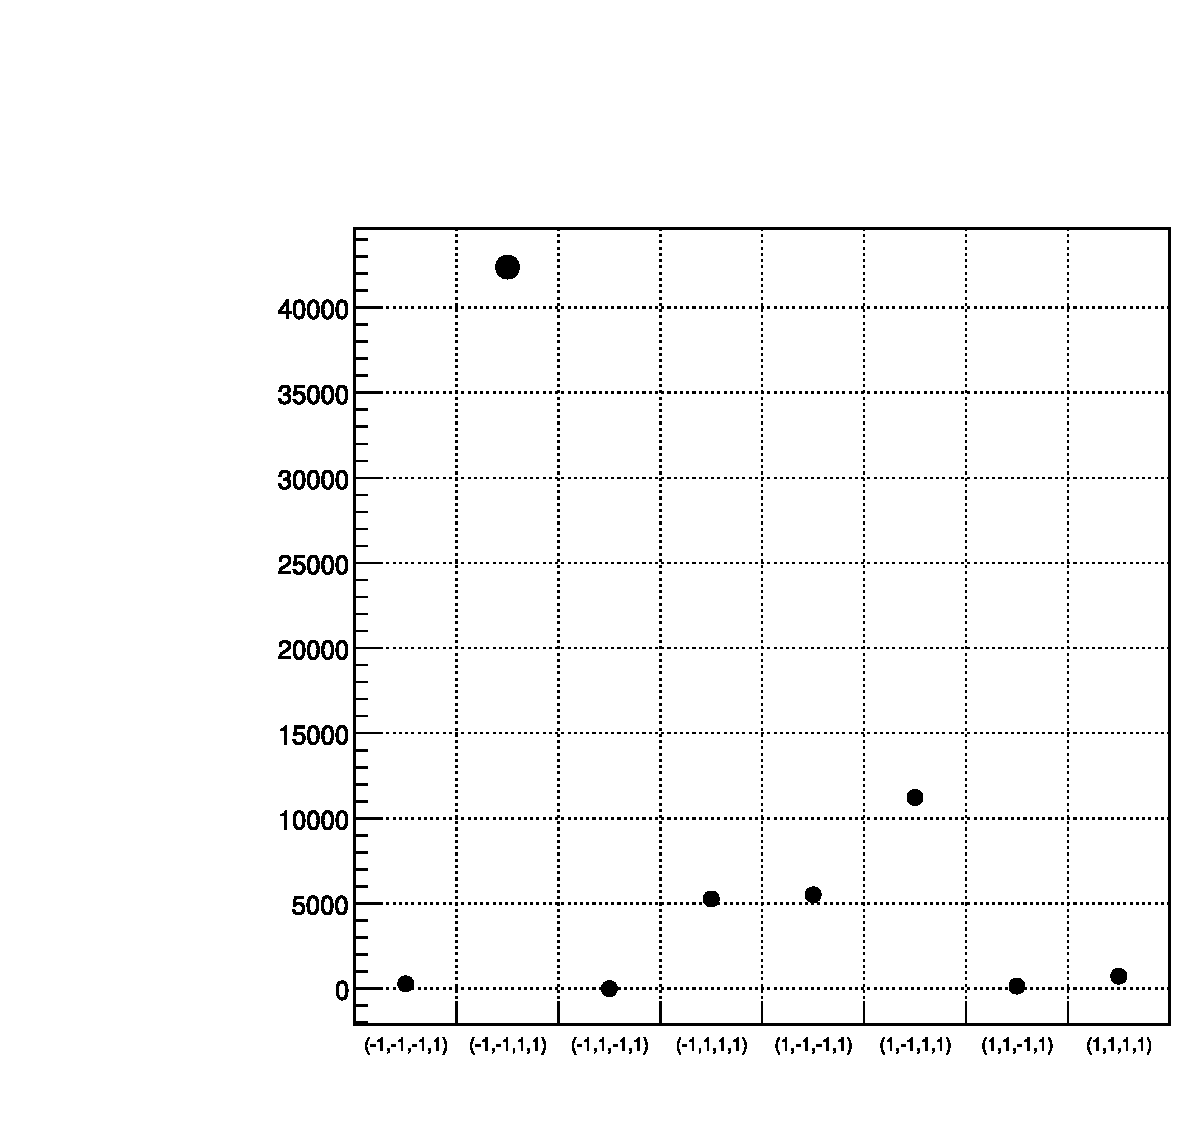
\includegraphics[width=\textwidth]{Pictures/10}
	\end{subfigure}
	\hspace{-1.5cm}
	\begin{subfigure}{0.375\textwidth}
		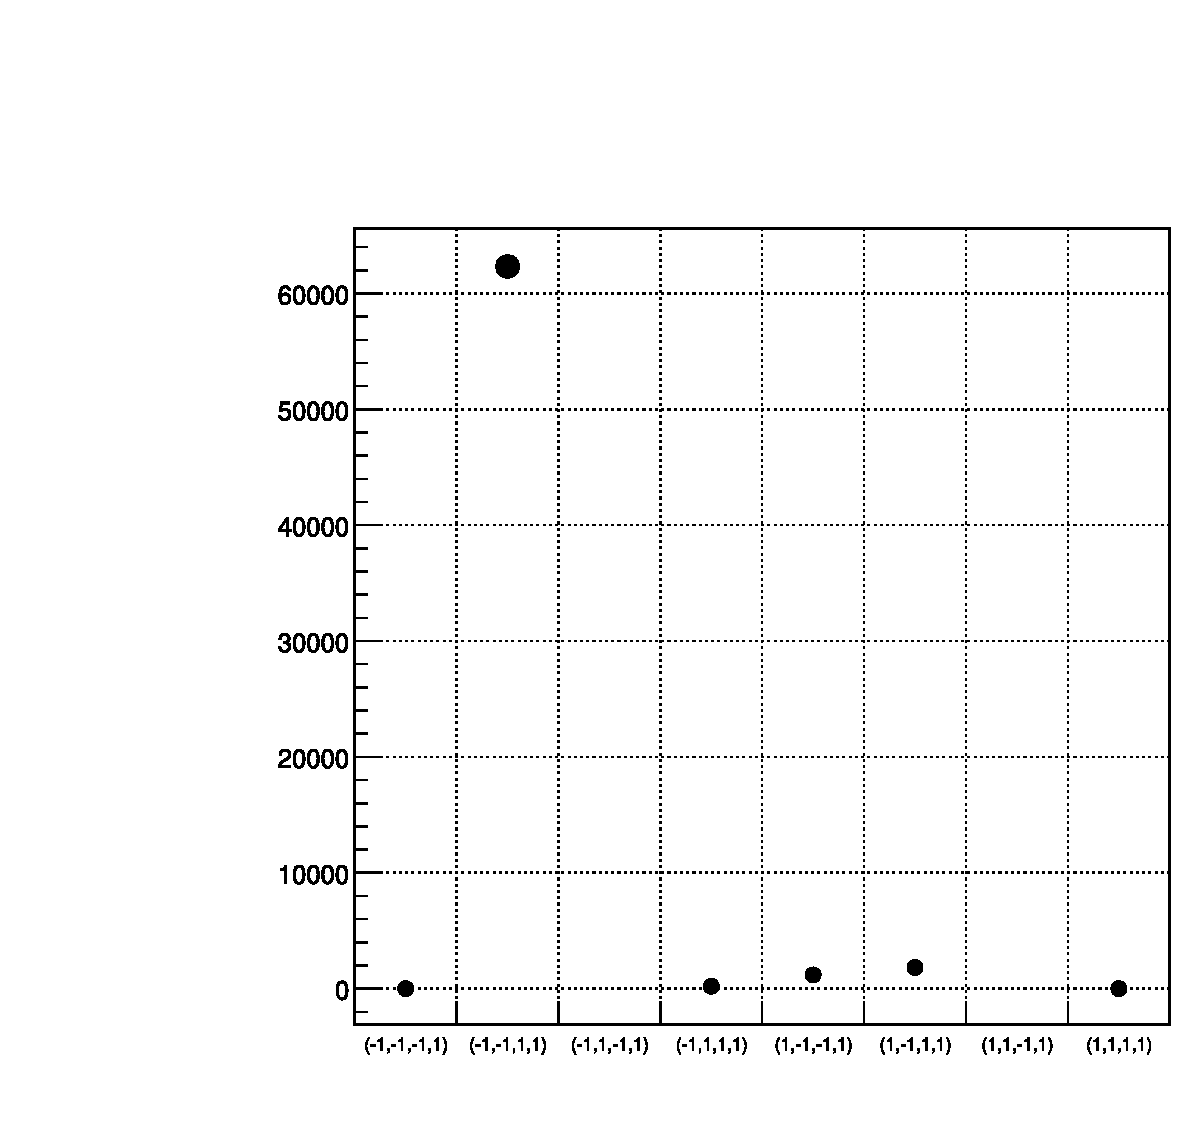
\includegraphics[width=\textwidth]{Pictures/11}
	\end{subfigure}
	
	\caption{Risultati}
	\label{fig:results}
\end{figure}
\restoregeometry

\end{document}
